
\documentclass{subfiles}

\begin{document}
	
\section{Problem and Challenges}\label{sec:Opt:Challenges}
{\color{blue}	
	\par While Section \ref{Visualisations} explains a simple approach of extracting a polygonal surface from the voxelised FW LiDAR data, this section is mainly focused on objective No. 5 from table (\ref{tab:Objectives}); it tests how well different data structures performs on the surface reconstruction and it attempts to improve the interpretation of volumetric data by introducing new data structures. The main challenges raised for this task are because the input data are real laser scanning data that contain noise. Some of the challenges that this chapter attempts to tackle are listed below:
  \begin{enumerate}
		\item The LiDAR sensors are vulnerable to clouds and seagulls being misinterpreted and recorded as hit points. Those outliers are much higher than tree canopies but they are within the boundaries of the scanned area. As a result, on average 96\% of the voxels are empty.   	
		\item Marching Cube is a scan line algorithm, which implies looping through every single voxel, including the empty ones. This is very time consuming and therefore, algorithms that quickly identify and ignore empty areas are essential. 
		\item While loading an entire volume, the huge amount of empty voxels may lead into exceed usage of memory. It is therefore preferable to store the voxels into a hierarchical structure that avoids storing the empty ones.
		\item When extracting a surface from real data, it is very likely to generate non-manifold objects. Non-manifold objects are not homeomorphic to Euclidean 1-space because they have crossing points. This also occurs at the polygonal meshes generated by DASOS as explained at Chapter \ref{Visualisations}.
	\end{enumerate}

	
}

\section{Related work}
\subsection{Full-Waveform LiDAR Visualisation}

\par{\color{blue}Summarising previous aforemonetioned related work (Section \ref{LiDARsoftwares}), } traditional ways of interpreting the full-waveform LiDAR data suggest echo decomposition for detecting peak points and interpreting the point clouds extracted \cite{Wanger2006}. Both SPDlib \cite{Bunting2013} and FullAnalyse \cite{Chauve2009} visualises either the peak extracted points or the raw waveform samples. On the one hand, SPDlib visulises the samples as points with intensity above a given threshold, while FullAnalyse generates a sphere with radius directly correlated to that intensity of each wave sample. Similarly, Pulsewaves visualises a number of waveforms with different transparency according to their intensity \cite{Isenburg2012Pulsewaves}. {\color{blue}
On the one hand, visualising all the wave samples makes understanding of data difficult due to the high noise. On the other hand, peak point extraction identifies significant features but the FW LiDAR data also contain information about echoes width. These information can be accumulated from multiple shots into a voxel array, building up a 3D discrete density volume \cite{Miltiadou2014}.} 
\par Voxelisation of FW LiDAR data was introduced by \cite{Persson2005} who used it to visualise small scanned areas (15mx15m). The waveforms samples were inserted into a 3D Voxelised space and the voxels were visualised using different transparencies according to their intensity. Similarly, as explained at Section \ref{Voxelisation}, we adopt voxelisation for surface reconstruction and applied it on larger areas. Once the 3D density volume is generated, numerical implicitisation is used to represent the scanned area. Nevertheless, visualising numerical/implicit objects is not straight forward, since they contain no discrete values (Section \ref{sec:AlgebracObjects}). This problem can either be address by ray-tracing \cite{Hanrahan1983} or polygonisation \cite{Lorensen1987}. At this thesis, the polygonisation direction is taken, as explained in Section \ref{sec:SurfaceReconstruction}. This chapter introduces new ways of interpreting real voxelised data {\color{blue} and tests how well six data structures performs on surface reconstruction.} 


\subsection{Optimising Volumetric Iso-surface Extraction}
\par Even though volumetric visualisation has only been recently used for FW LiDAR systems, there are many applications in medical visualisation \cite{Levoy1998} \cite{Hadwiger2012} and visual effects \cite{Crassin2009} \cite{Laine2011SparseOctrees}. Research work exists on optimising both ray-tracing and surface reconstruction and it can be categorised into three groups: surface-tracking, parallelisation and data structures. Those approaches are discussed below along with their benefits and limitation in respect to voxelised FW LiDAR data.

\par Surface-tracking was applied at \cite{Rodrigues2005} \cite{Hartmann1998}. Starting from a seed point, the surface is expanded according to the local curvature of the implicit object. This method is considered to be faster and more efficient in comparison to the Marching Cubes algorithm since huge empty spaces are ignored. It further opens up possibilities for finer surface reconstruction at areas with high gradient changes. Nevertheless, surface-tracking algorithms cannot be applied with real laser scanning data because these data are neither manifold or closed. For example in a forest scene, a tree may be detached from the ground due to missing information about its trunk.Therefore by tracking the surface, the algorithm may converged at a single tree instead of the entire forest.  

\par Hansen and Hinker proposed parallelising the polygonisation process of BlobTree trees on Single Instruction, Multiple Data (SIMD) machines \cite{Hansen1992}. On SIMD machines greater speed up is achieved at longer instruction. BlobTree trees represent implicit objects as a combination of primitives and operations \cite{Galbraith2004}. While the depth of the tree increases, the lenght of the instruction increases as well. Nevertheless the fuction at the implicit representation of the FW LiDAR data at \cite{Miltiadou2014} is executed at constant time, making it harder to achieve speed up using SIMD machines. Further, according to the C++ Coding Standards when optimisation is required is better to seek an algorithmic approach first because it is simpler to maintain and less likely to contain bugs \cite{Sutter2004}. 


\par {\color{blue}Hierarchical data structures, like octrees, improves the performance of the isosurface extraction because of the huge amount of empty voxels that can be ignored during polygonisation \cite{Wilhelms1990}. The literature in the data structures direction aims to either simplify/improve the output mesh, optimise traversal time of hierarchical data structures or eliminate hierarchy. For example, the extraction of locally finer details either with dual grids \cite{Scott2005} or edge-trees \cite{Wilhelms1992} reduces the amount of vertices produced. In addition, a net of linked surface nodes improved anti-aliasing and reduces artifacts of 3D Magnetic Resonance Imaging (MRI) \cite{Gibson1998}. Regarding efficiency of accessing data, } franctional cascading slightly improved time complexity of range queries\cite{Chazelle1986}. Sparse Voxel Octrees improved efficiency by having a pointer pointing to children and packing children coherently in memory \cite{Laine2011SparseOctrees}. Hadwiger et al uses a 3D virtual memory to keep voxels coherent on GPU and avoid traversal \cite{Hadwiger2012}. Nevertheless, due to the adjacency of neighbouring voxels, data are saved for empty voxels yielding into much wasted memory. OpenVDB library arranges blocks of grids into a B+ hierarchical data structure for increased cache coherency and lower tree depth \cite{Museth2013OpenVDB}. The bricks stuctured used at GigaVoxels is similar in terms of blocks, named bricks, and it's been used for efficient GPU ray-casting \cite{Crassin2009}. For eliminating tree traversal time, Warren and Salmon introduced hash octrees for N-bosy simulation of particles \cite{Warren1993hashedOctree}. Similarly, voxel hashing was proposed for overheading the traversal time of hierarchical structures and real time surface reconstruction was achived using depth cameras online \cite{Nievner2016voxelHashing}. Most of those data structure optimisations are based on GPU processing, but they are still very relevant.


\section{Overview}

{\color{blue}

\par This thesis compares six approaches for handling and polygonising voxelised full-waveform LiDAR data. The first three approaches use data structures from the literature and the scan line Marching Cubes algorithm. An explanation of their functionalities is given at Table \ref{tab:DataStructuresScanline}. The last three approaches are more complicated because they take into consideration the chunks of empty voxels and ignore them during surface reconstruction. A brief summary of them is given in Table \ref{tab:DataStructuresOptimised} and they are fully explained in Section \ref{sec:Opt:Methods}. Please note that the "1D Array" is the original implementation, while each one of the other five approaches tackles at least one of the aforementioned challenges (Section \ref{sec:Opt:Challenges}). 

}

\begin{table}[!htbp]
	% increase table row spacing, adjust to taste
	\renewcommand{\arraystretch}{1.3}
	% if using array.sty, it might be a good idea to tweak the value of
	% \extrarowheight as needed to properly center the text within the cells
	
	\centering
	% Some packages, such as MDW tools, offer better commands for making tables
	% than the plain LaTeX2e tabular which is used here.
	\begin{tabular}{|P{0.3\textwidth}|P{0.3\textwidth}|P{0.3\textwidth}|}
			
		\hline
		\textbf{1D Array} &	\textbf{Voxel Hashing} & \textbf{Octree}  \\
		\hlinewd{1.5pt}
		{\color{blue}Influenced by \cite{Hadwiger2012}, all the data are saved into an 1D array to guarantee coherent memory, even though much memory is wasted in regards of empty voxels.} &	{\color{blue}The intensities of the voxels are saved into a simple hash table with key value relevant to their position into the volume. Similary to \cite{Nievner2016voxelHashing}, this approach overheads traversing time of hierarchical structures and on top of that it reduces memory allocation because empty voxels are not stored. } & {\color{blue} This is a traditional  hierarchical octree with traversal time to be essential. Please note that this is a scan line test and therefore it does not take into consideration empty chunks of memory.}\\	
		\hline
	\end{tabular}
	\caption{Brief Description of the Three Scan-Line Tests}
	\label{tab:DataStructuresScanline}
\end{table}



\begin{table}[!htbp]
	% increase table row spacing, adjust to taste
	\renewcommand{\arraystretch}{1.3}
	% if using array.sty, it might be a good idea to tweak the value of
	% \extrarowheight as needed to properly center the text within the cells
	
	\centering
	% Some packages, such as MDW tools, offer better commands for making tables
	% than the plain LaTeX2e tabular which is used here.
	\begin{tabular}{|P{0.3\textwidth}|P{0.3\textwidth}|P{0.3\textwidth}|}	
		\hline
		\textbf{Integral Volumes} &	\textbf{Octree Max and Min} & \textbf{Integral Tree}  \\
		\hlinewd{1.5pt}
		{\color{blue} This data structure is an extension of Integral Images to 3D. It was firstly presented at the CGVC conference and it is a part of this thesis. Using Integral Volumes, the sum of any cuboid area is calculated in constant time. By repeatedly dividing the space into cuboids, big empty spaces are quickly identified and ignored during the surface reconstruction. \newline(Section \ref{sec:IVopt}) }&	{\color{blue}In this approach, the values are saved into an octree, but the surface reconstruction is build along the tree. This is slightly different than a traditional octree, because at each branch node its max and min values are saved. This way, areas that are completely full or empty are identified during traversal before reaching the leaves of the trees. (Section \ref{sec:OctreeMaxMin}) } &{\color{blue} It is a combination of Octree and Integral where the sum of a given branch is returned at constant time. That was an attempt to combine the idea of Integral Images and Octrees. Nevertheless, traversal time and backtracking for finding neighbouring voxels still exists. (Section \ref{sec:ITopt})}\\	
		\hline
	\end{tabular}
	\caption{Description of the Three Optimisation Attempts}
	\label{tab:DataStructuresOptimised}
\end{table}

\newpage
\section{The Optimisation Methods}\label{sec:Opt:Methods}

\section{Integral Volumes}\label{sec:IVopt}
The Integral Volumes optimisation is based on the idea of Integral Images, which is an image representation where each pixel value is replaced by the sum of all the pixels that belong to the rectangle defined by the lower left corner of the image and the pixel of interest.  An integral image is constructed in linear time and the sum of every rectangular area is calculated in constant time, as shown in figure \ref{fig:IntegralImages} \cite{Crow1984}


\begin{figure}[!htbp]
	\centering
	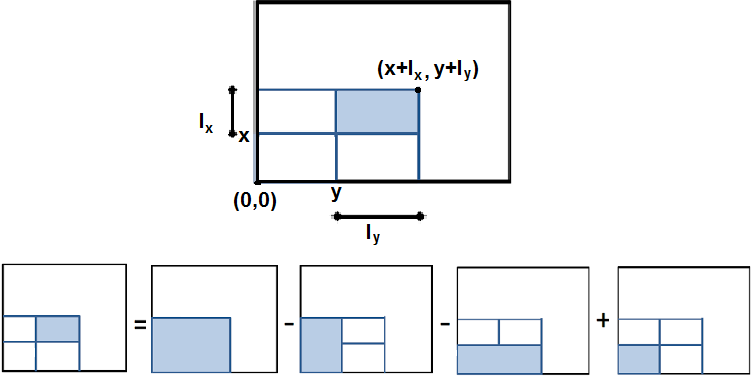
\includegraphics[width=5.5in]{img/IntegralImages}
	% where an .eps filename suffix will be assumed under latex, 
	% and a .pdf suffix will be assumed for pdflatex; or what has been declared
	% via \DeclareGraphicsExtensions.
	\caption[Integral Image]{Once the Integral Image is constructed, the sum of any rectangular area is calculated in constant time.}
	\label{fig:IntegralImages}
\end{figure}


In this paper, we extend Integral Images to Integral Volumes and use them to quickly identify and ignore big chunks of empty voxels during polygonisation. The following section explains the mathematics behind Integral Volumes, while sections \ref{sec:IVoptApproach}  and \ref{sec:IVcodeDetails} give an in depth description about the algorithms invented. 

\subsection{Extending Integral Images to Integral Volumes}\label{sec:extendingIV}

As shown in Figure \ref{fig:IntegralImages},the area of interest is defined by the pixels $(x, y)$ and $(x+l_x, y+l_y)$ and the sum $S$ is given by: 
\begin{equation}
\begin{split}
S = & T(x+l_x,y+l_y) - 
T(x+l_x,y-1)- \\
&  T(x-1,y+l_y) +
T(x-1,y-1)
\end{split}
\label{eq:IntegralImage}
\end{equation}

where 	$S$ is the sum of rectangular area of interest, $T(x, y)$ is the value of the integral image at $(x, y)$ and $l_x, l_y$ define the length of the rectangle in the x and y axis respectively. 

Extending integral images to 3D, the value of the voxel $(x ,y, z)$ in a 3D integral volume becomes equal to the sum of all the values that belong to the box defined by the $(x, y, z)$ and $(0, 0, 0)$ included. 
Therefore the sum $(S)$ of the box defined by $(x, y, z)$ and $(x+l_x, y+l_y, z+l_z)$ included is given by:
\begin{equation}
\begin{split}
S = & T(x-l_x,y+l_y,z+l_z) - 
T(x-1,y+l_y,z+l_z) - \\
&  T(x+l_x,y-1,z+l_z) - 	
T(x+l_x,y+l_y,z-1) + \\
&  T(x-1,y-1,z+l_z)   +
T(x-1,y+l_y,z-1)   +  \\
&  T(x+l_x,y-1,z-1)   -
T(x-1,y-1,z-1)
\end{split}
\end{equation}

where 	$T(x, y, z)$ is the value of the voxel $(x, y, z)$ in the 3D integral volume.  
$S$ is the sum of voxels inside the box, $T(x, y, z)$ is the value of the voxel $(x, y, z)$ in the 3D integral volume. and $l_x, l_y, l_z$ define the length of the box in the $x$, $y$ and $z$ axis respectively. 



\subsection{Optimisation Algorithm}\label{sec:IVoptApproach}
As mentioned before, using Integral volumes empty areas are quickly identified and ignored during polygonisation. An iterative algorithm is introduced here. This algorithm continuously splits the volume and checks whether the sub-volumes and its neighbouring voxels are empty using the Integral Volumes. Please note that all the values below the threshold boundary of the object must be zero and all the non-empty voxels must contain a positive value.  

\begin{algorithm}
	\caption{Integral Volumes Optimisation Algorithm}
	\label{alg:IVoptSimple}
	\centering
	\begin{algorithmic}[1]
		\State Push the entire Volume as a cuboid inside a Stack
		\While {stack is not empty }
		\State Cuboid-A   $\gets$  next cuboid from the Stack 
		\If{Cuboid-A and neighbours are empty} 
		\State	discard Cuboid-A
		\ElsIf { Cuboid-A consists of only one cube}
		\State polygonise Cuboid-A
		\Else 
		\State divide Cuboid-A
		\State push the two new Cuboids into stack
		\EndIf
		\EndWhile
	\end{algorithmic}
\end{algorithm}
Here it is worth highlighting that, on line 3 of the algorithm it is checked if the neighbouring cubes of a cuboid are empty, because the voxels of the 3D density volume and the cubes in marching cubes algorithm are  aligned with an offset (Figure \ref{fig:ExpectedSampling}). If volumes with non-empty neighbouring voxels are ignored, then holes appear on the output polygon mesh. 		

\begin{figure}[!htbp]
	\centering
	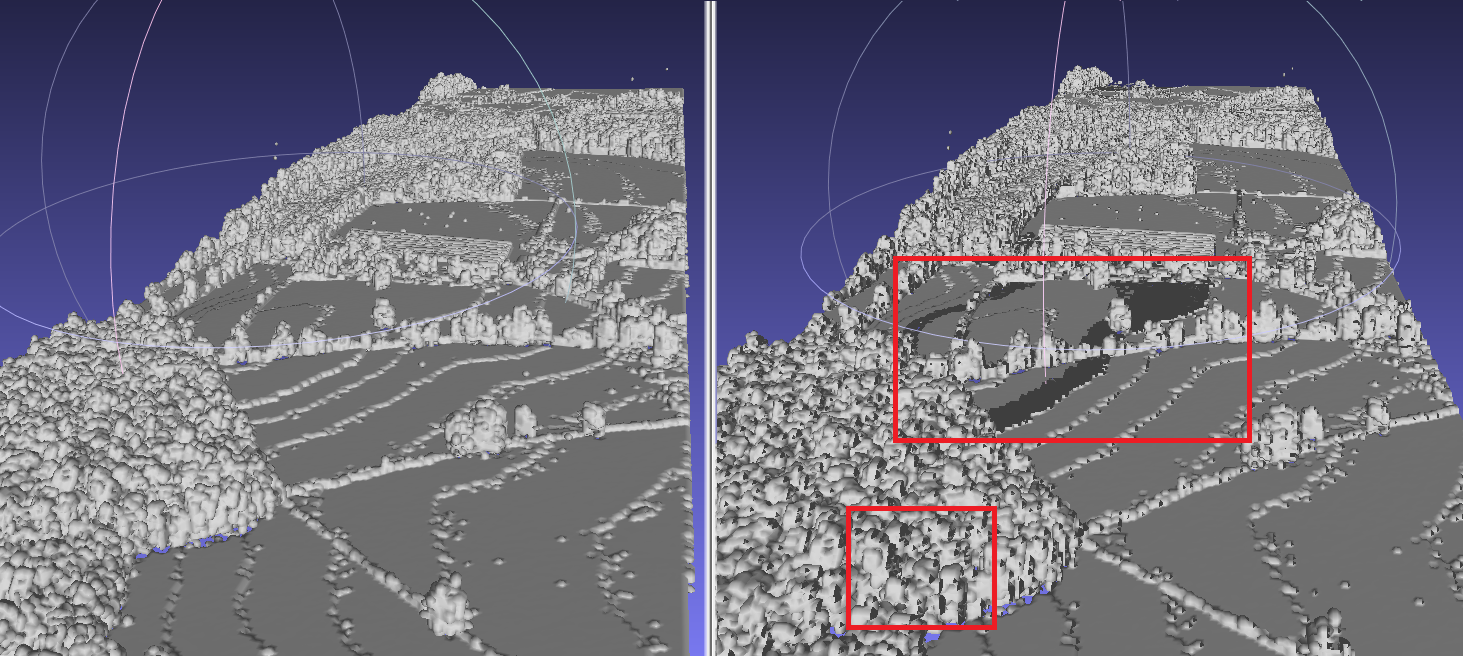
\includegraphics[width=5.5in]{img/HolesNeighbours}
	% where an .eps filename suffix will be assumed under latex, 
	% and a .pdf suffix will be assumed for pdflatex; or what has been eclared
	% via \DeclareGraphicsExtensions.
	\caption{Comparison between including and ignoring neighborouing voxels; holes appears when ignored.}
	\label{fig:IVholesNeighbours}
\end{figure}

\subsection{Coding Details for Faster Implementation}\label{sec:IVcodeDetails}
Implementation details contributes to the efficiency and speed up of the algorithm. Significant improvements are achieved by reducing recursions, big memory allocations and if statements, since memory jumps are time expensive. As shown in algorithm \ref{alg:IVoptSimple}, a while loop is used to avoid recursion. In this section it's given an explanation on how the stack controls memory consumption and how bitwise operations reduces if-statement usage. 

Regarding memory consumption, a stack was chosen over a queue, to decrease the amount of cubes saved into the data structure simultaneously. A queue is a first in first out data structure, while a stack accesses data in a last in first out order. In every iteration, it is ideal to interpret the smallest saved cube, such that the possibility of being polygonised is higher and the possibility of storing another cube is less. A queue guarantees cubes with approximately the same size, since the big cubes will be added first and sequentially being divided first. In contrast, a stack guarantees the smallest possible number of cubes saved. The larger cubes are stored in the bottom of the stack while the smaller ones are interpreted first because they are always the last one divided and inserted into the stack.  For that reason, a stack guarantees the lowest memory usage. 

Furthermore, in algorithm \ref{alg:IVoptSimple} an issue exists: how to quickly identify the side to be divided next? Ideally, the usage of if-statements should be low because they contains many time expensive memory jumps. For that reason, bitwise operations were embedded into the program to reduce their usage. A cube is defined with its position, its size, the next side to be divided $s$ and its divisible sides $D$. The parameter $s$ takes the values $1$, $2$, $3$ for the $x$, $y$, $z$ sides respectively. The parameter $D$ is an integer consisting of the sum of three numbers $(1$ or $0)+(2$ or $0)+(4$ or $0)$ indicating whether the sides  $x$, $y$, $z$ are divisible or not (table \ref{tab:divisiblesNum}). The parameter $D$ takes the value between $[0,7]$ and covering all the possible cases of divisible sides as shown in tables \ref{tab:Dnumbers} and \ref{tab:Dbinary}. For example if $x$ and $z$ are the divisible sides, then $D = 1+0+4 = 5$. By the end, the bitwise operations and the faster implementations of the Integral Volumes optimisations is shown at algorithm \ref{alg:IVoptAdvance}.



\begin{table}[!htbp]
	% increase table row spacing, adjust to taste
	\renewcommand{\arraystretch}{1.3}
	% if using array.sty, it might be a good idea to tweak the value of
	% \extrarowheight as needed to properly center the text within the cells

	\centering
	% Some packages, such as MDW tools, offer better commands for making tables
	% than the plain LaTeX2e tabular which is used here.
	\begin{tabular}{|P{1.4cm}||P{1.4cm}|P{1.4cm}||P{1.4cm}|P{1.4cm}|}	
		\hline
		&	\multicolumn{2}{c||}{Decimal Numbers} & \multicolumn{2}{c|}{Binary Numbers}  \\
		\hline\hline
		Side &	Divisible & Not\newline Divisible &	Divisible &	Not \newline Divisible  \\
		\hline
		X &	1 &	0 &	0001 &	0000  \\	
		\hline
		Y &	2 &	0 &	0010 &	0000  \\
		\hline
		Z &	4 &	0 &	0100 &	0000 \\
		\hline
	\end{tabular}
	\caption{Values of divisible sides}
	\label{tab:divisiblesNum}
\end{table}



\begin{table}[!htbp]
	% increase table row spacing, adjust to taste
	\renewcommand{\arraystretch}{1.3}
	% if using array.sty, it might be a good idea to tweak the value of
	% \extrarowheight as needed to properly center the text within the cells
	\centering
	% Some packages, such as MDW tools, offer better commands for making tables
	% than the plain LaTeX2e tabular which is used here.
		\begin{tabular}{|P{0.7cm}||P{0.7cm}|P{0.7cm}|P{0.7cm}|P{0.7cm}|P{0.7cm}|P{0.7cm}|P{0.7cm}|P{0.7cm}|}	
		\hline
		X &	1 &	- &	1 &	- &	1 &	- &	1 &	- \\	
		\hline
		Y &	2 &	2 &	- &	- &	2 &	2 &	- &	- \\
		\hline
		Z &	4 &	4 &	4 &	4 &	- &	- &	- &	- \\
		\hline
		D &	7 &	6 &	5 &	4 &	3 &	2 &	1 &	0 \\
		\hline
	\end{tabular}
	\caption{How to calculate the value of D, which represents the divisible sides of a cuboid}
	\label{tab:Dnumbers}
\end{table}


\begin{table}[!htbp]
	% increase table row spacing, adjust to taste
	\renewcommand{\arraystretch}{1.3}
	% if using array.sty, it might be a good idea to tweak the value of
	% \extrarowheight as needed to properly center the text within the cells
	\centering
	% Some packages, such as MDW tools, offer better commands for making tables
	% than the plain LaTeX2e tabular which is used here.
	
	\begin{tabular}{|P{0.7cm}||P{0.7cm}|P{0.7cm}|P{0.7cm}|P{0.7cm}|P{0.7cm}|P{0.7cm}|P{0.7cm}|P{0.7cm}|}
		\hline
		X &	0001 &	-	 &	0001 &	-	 &	0001 &	-	 &	0001 &	-   \\
		\hline
		Y &	0010 &	0010 &	-	 &	-	 &	0010 &	0010 &	-	 &	-   \\
		\hline
		Z &	0100 &	0100 &	0100 &	0100 &	-	 &	-	 &	-	 &	-   \\
		\hline
		D &	0111 &	0110 &	0101 &	0100 &	0011 &	0010 &	0001 &	0000\\
		\hline
	\end{tabular}
	
	\caption{How to calculate the value of divisible sides (D) in binary representation}
	\label{tab:Dbinary}
\end{table}



\begin{algorithm}[!htbp]
	\caption{Integral Volumes Optimisation Algorithm}
	\label{alg:IVoptAdvance}
	\centering
	\begin{algorithmic}[1]
		\State Push the entire Volume as a cuboid inside a Stack
		\While {stack is not empty }
			\State Cuboid-A   $\gets$  next cuboid from the Stack 
			\If{Cuboid-A and neighbours are empty} 
				\State	discard Cuboid-A
			\ElsIf { $D$ is equal to $0$}
				\State polygonise Cuboid-A
			\ElsIf { $( D$ bitwise add $2^s )$ shift right $(s-1)$ }
				\State	divide side s of Cuboid-A 
		
				\If { the new length of side $s$ is equal to $1$ } 
					\State	$D \gets D$ bitwise add $(7-2^s)$
				\EndIf
				\State 	$s \gets (s+1) \text{ mod } 3$
				\State push both new Cuboids into stack
			\Else 
				\State $s \gets (s+1) \text{ mod } 3$
				\State push Cuboid-A back into the stack
			\EndIf
		\EndWhile
	\end{algorithmic}
\end{algorithm}

\newpage

\rhead{ }
\section{Octree Max and Min {\color{red} **Everything from here is new :)}} \label{sec:OctreeMaxMin}

\par Integral Volumes quickly identify and ignore empty spaces during polygonisation (tackles the 1st, 2nd and 4th problem of the original algorithm -- Section \ref{sec:Opt:Challenges}), but it allocates memory for the entire volume (the 3rd problem). For that reason, the `Octree Max and Min' data structure has been implemented. 

\par The `Octree Max and Min' data structure avoids storing empty voxels and it also identifies empty areas during polygonisation. The polygonisation is built on the traversal of the octree, as explained in Algorithm \ref{alg:MCOctree}. Similarly to Integral Volumes, a stuck is used to avoid recursion and reduce memory jumps. While using the Integral volumes, it is checked whether the neighbours of a cuboid is empty or not to avoid generating holes on the polygonal mesh. This is also essential when a branch to be discard at 'Octree Max and Min' data structure. But because the every branch of an octree is cubic and power of two, it is not trivial to check whether the neighbours of a branch are empty or not. For that reason, we loop through its edges and polygonise them according to look up table of the the Marching Cubes algorithm. 


\begin{algorithm}[!htbp]
	\caption{Embedding the Marching Cubes Algorithm into an octree structure}
	\label{alg:MCOctree}
	\centering
	\begin{algorithmic}[1]
		\State Push the Root as a Node into a Stack
		\While {stack is not empty }
		\State Node-N   $\gets$  next Node from the Stack 
		\If{ Node-N is a Leaf}
		\State polygonise Leaf
		\ElsIf{Node-N has no children OR max value of Node-N < isolevel \newline OR min value of Node-N > isolevel} 
		\State	POLYGONISE\_EDGES\_OF\_CUBIC\_WITH\_ROOT\_NODE-N()	
		\Else
		\State push the children of Node-N into the Stack
		\EndIf
		\EndWhile
	\end{algorithmic}
\end{algorithm}




\par Embedding the polygonisation of volumetric data into an octree has been done before \cite{Wilhelms1990}. Nevertheless, the 'Octree Max and Mean' data structure differs in two ways:
\begin{itemize}
	\item The max and min values of each branch are stored into the corresponding node to speed up polygonisation. This enables checking whether the leaves of a branch lie either only inside or only outside the implicit object{\footnote{Explanation about implicit/algebraic objects is given at Section \ref{sec:AlgebracObjects}}}. If they do, then no iso-surface is crossing that branch and it can be discarded (after polygonising its edges).
    \item A new algorithm is proposed and implemented for finding neighbouring voxels. This algorithm reduces comparisons and jumps in memory. An in-depth explanation of this algorithm is given at Section \ref{sec:NeighboursFinding}.
\end{itemize}





\subsection{Finding Neighbours}\label{sec:NeighboursFinding}

\par Every time a voxel/leaf is polygonised, seven of its neighbours are checked to decide whether a surface is passing through that area or not. At hierarchical data structures, the nearest common ancestor is tracked upwards and the branch, with root the common ancestor, is traversed to reach the neighbour. The article \cite{Hanan1989} uses recursion that terminates once a common ancestor between a leaf and its neighbour is identified. According to Scharack \cite{Schrack1992}, finding neighbours in linear octree \footnote{Linear octrees are octrees stored into a 1D-array instead of a hierarchical structure.} is done in constant time. Nevertheless, linear Octrees are full octrees. Therefore, if used in our case all the empty voxels would have to be stored as well. Lohner suggested vectorising the space during post-processing for finding the shorter distance between un-constructed points \cite{Lohner1994}. However, the 3D voxelised FW LiDAR is a regular grid and during polygonisation the shorter distance to travel is one voxel. For that reason simpler approaches with less initialisation time, like \cite{Schrack1992} could perform equally well. Castro et al. \cite{Castro2008} assume that with hierarchical octrees it is not possible to start searching neighbours from leaves and suggest using hashed octrees to do that. In contrast, it is possible to start from the leaves and find the common ancestor using parentship as described at \cite{Hanan1989}.

\par To avoid recursion and reduce comparison, this thesis introduces a new way of finding the  common ancestor using logarithms of $2$. The Algorithm \ref{alg:Ascestor} explains the proposed method. As shown in Figure \ref{fig:OctreeNeighbours}, there are occasions where it is cheaper to start searching a neighbour from the root instead of the leaf. For example Node-$F$ is the $(+1)$ neighbour of Node-$E$. If we start looking for it from the leaves then we need to travel through 6 nodes, but if we start from the root we only need to travel 5 nodes. Logarithms helps us decide which route to take, while reducing comparisons (i.e. no need to check whether branches has common faces while travelling upwards\cite{Hanan1989}).

\begin{algorithm}[!htbp]
	\caption{Finding the number of steps required to go upward in order to find the common ancestor of a Leaf$(x)$ of interest and it $(+1)$ neighbour}
	\label{alg:Ascestor}
	\centering
	\begin{algorithmic}[1]
		\State $c $  $\gets$ ceil$(log_2 x)$
		\State $c_1 \gets$ ceil$(log_2 (x+1))$
		\While {$c = c_1$}
		\State $x = x - 2^{(c-1)} $
		\State $c $  $\gets$ ceil$(log_2 x)$
		\State $c_1 \gets$ ceil$(log_2 (x+1))$		
		\EndWhile
		\If {$D_{max}/2 < c_1 $}
		\State Start from Root to find Neighbour Branch +1
		\Else
		\State Backtrack $c_1$ parents to find the common ancestor
		\State Find neighbour
		\EndIf
	\end{algorithmic}
\end{algorithm}

\begin{figure}[!htbp]
	\centering
	\includegraphics[width=5.5in]{img/OctreeNeighbours}
	% where an .eps filename suffix will be assumed under latex, 
	% and a .pdf suffix will be assumed for pdflatex; or what has been eclared
	% via \DeclareGraphicsExtensions.
	\caption{This diagram depicts the parameters used for finding neighbouring voxels.}
	\label{fig:OctreeNeighbours}
\end{figure}


\newpage

\section{Integral Tree}\label{sec:ITopt}
\par 

\subsection{Main Idea }

\par The Integral Tree is a new term that describes the attempt to preserve some properties of the Integral Images while using a non-full tree structure. Every Integral Tree consists of two elements: an integral 1D-array and a tree. All the values of every non-empty and non-connecting node are saved into an 1D-array, in a way such that the Integral Tree's condition is fulfil: all the values of every branch $B$ are adjacent inside the 1D-array. Afterwards the array is converted to integral; the sum of every $n$ continuous values is calculated in constant time. Additionally, the root node of each branch $B$ contains two parameters $(*p, k)$. The number $k$ is the number of nodes with values the branch $B$ has (e.g. for an octree, it is all its leaf nodes) and the pointer $*p$ points to the first one in the 1D-array (Figure \ref{fig:IntegralTreeMainIdea}).

\begin{figure}[!htbp]
	\centering
	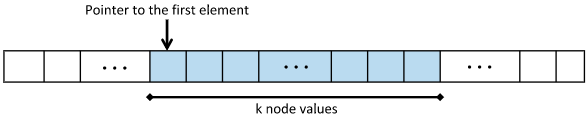
\includegraphics[width=5.5in]{img/IntegralTreeMainIdea}
	% where an .eps filename suffix will be assumed under latex, 
	% and a .pdf suffix will be assumed for pdflatex; or what has been eclared
	% via \DeclareGraphicsExtensions.
	\caption{Ordering of tree elements}
	\label{fig:IntegralTreeMainIdea}
\end{figure}

\par The aforementioned rules can be applied to any tree structures including binary trees, quadtrees and octrees. To better perceive how this data structure works, let’s assume that there is a number of 2D spatially distributed values. Figure  \ref{fig:IntegralTreeQuads} depicts how they can be saved into an Integral Quad Tree in order to fulfil the Integral Tree's condition of adjacency. Also, Section {\ref{sec:IntegralBinaryTree}} gives an example of an Integral Binary Tree.

\begin{figure}[!htbp]
	\centering
	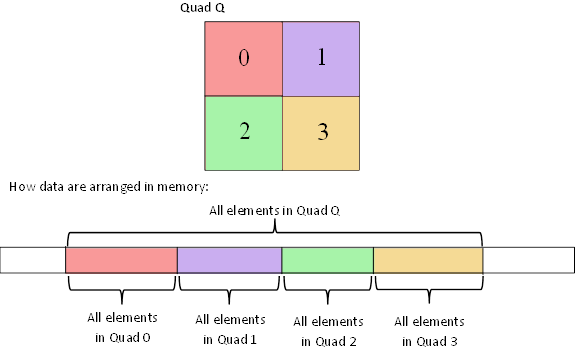
\includegraphics[width=5.4in]{img/IntegralTree}
	% where an .eps filename suffix will be assumed under latex, 
	% and a .pdf suffix will be assumed for pdflatex; or what has been eclared
	% via \DeclareGraphicsExtensions.
	\caption{Illustration of how to save the values of an Integral Quad Tree into the 1D-array, in order to preserve the condition of Integral Trees}
	\label{fig:IntegralTreeQuads}
\end{figure}


\subsection{Integral Binary Tree Example}\label{sec:IntegralBinaryTree}

\begin{figure}[!htbp]
	\centering
	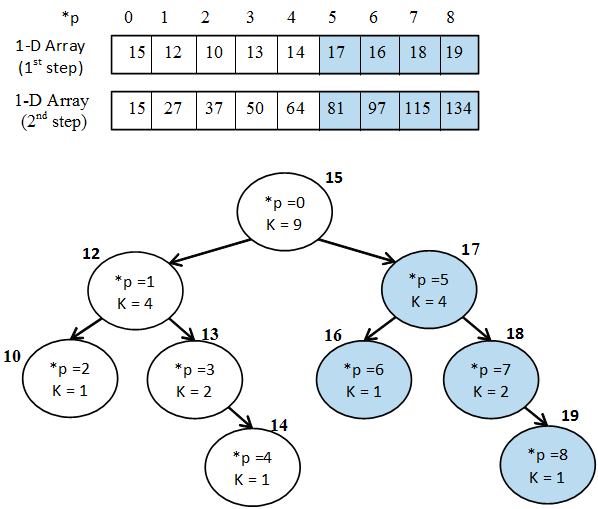
\includegraphics[width=4.8in]{img/IntegralBinaryTree}
	% where an .eps filename suffix will be assumed under latex, 
	% and a .pdf suffix will be assumed for pdflatex; or what has been eclared
	% via \DeclareGraphicsExtensions.
	\caption{Example of Integral Binary Tree}
	\label{fig:IntegralBinaryTree}
\end{figure}

\par  An example of applying the idea of Integral Tree into a binary tree is given for clarity (Figure \ref{fig:IntegralBinaryTree}). Firstly, the values of the binary tree are sorted into the 1D-array $A$ as $\{15,$ $12,$ $10,$ $13,$ $14,$ $17,$ $16,$ $18,$ $19\}$ in order to fulfil the Integral Tree's condition of adjacency. Secondly, the array $A$ is modified as $\{15,$ $27,$ $37,$ $50,$ $64,$ $81,$ $97,$ $115,$ $134\}$ in order to become integral using the following equation:

\begin{equation}
\begin{split}
A[i]=A[i]+A[i-1]
\end{split}
\end{equation}


\par Then, the sum $S$ of each branch with root $*p$ and $k$-nodes is calculated at constant time as follow:


\begin{equation}
\begin{split}
S = A[*p+k-1]-A[*p-1]
\end{split}
\end{equation}

\par For instance the sum of the blue branch on Figure \ref{fig:IntegralBinaryTree} is $A[5+4-1]-A[5-1] = A[8]-A[4] = 134-64 = 70$, which is correct since $17+16+18+19=70$.




\subsection{Integral Octree for Surface Reconstruction}

The same algorithms as 'Octree Max and Min' are used. The only difference is at the comparison of Line 6 at Algorithm \ref{alg:MCOctree}. 

at octree the values saved into the 1-D array are all the leaves of the trees. 




The leaves of the octree are saved into the 1D-array. 




\section{Results and Discussion}

The following tests first test how well each data structure performs in terms of execution time and memory usage. 
Different algorithms could either be beneficial in speeding up the process or decrease memory usage. 


Time program required to be executed
Table single flightline different resolutions



Same resolution, constant noise level, different Flightlines



LDR-FW-FW10\_01-201009821.LA



On the one hand, it preserves the lower memory consumption of an octree, but despite Integral Volumes, when using an octree the space should be cubic and finding neighbouring voxels is more complicated and time consuming. 

More complicated to pre-save values for faster interpolation. 

The Hashed Octree approach could further be used for speeding up neighbouring search in spatial representation of geometric objects.

By the end, even though this new data structure is extremely beneficial for the aforementioned optimisation algorithm (Section 4.4***) and multi-resolution direct volumetric rendering, there is a big drawback associated with it: adding elements to it implies reconstruction of the entire tree. In volumetric rendering of FW LiDAR data, the possibility of adding new elements in the volume is not big and the data of each scan are constant, so this is not a considerable problem for this project. Nevertheless, in the case of cloud simulation in animated movie, this structure would have not been appropriate due to the time required to reconstruct the tree every time an element is added or modified. 


{
\begin{sidewaystable}[!htbp]
	\small
	% increase table row spacing, adjust to taste
	\renewcommand{\arraystretch}{1.3}
	% if using array.sty, it might be a good idea to tweak the value of
	% \extrarowheight as needed to properly center the text within the cells
	\centering
	% Some packages, such as MDW tools, offer better commands for making tables
	% than the plain LaTeX2e tabular which is used here.
	\begin{tabular}{|P{1.75cm}|P{2.1cm}||P{0.82cm}|P{0.85cm}|P{0.9cm}|P{0.7cm}||P{0.7cm}|P{0.97cm}|P{0.97cm}|P{0.7cm}||P{0.7cm}|P{1cm}|P{1cm}|P{0.7cm}|}	
    \hlinewd{1.5pt}
		\multicolumn{2}{|c||}{} & \multicolumn{4}{c||}{\textbf{1D-Array}} & \multicolumn{4}{c||}{\textbf{Voxels Hashing}} &\multicolumn{4}{c|}{\textbf{Octree}}  \\
		\hline
		
		\multicolumn{2}{|c||}{Resolution} & \multicolumn{3}{c|}{Time (s)} & \multicolumn{1}{c||} {Memory} & \multicolumn{3}{c|}{Time (s)}&  \multicolumn{1}{c||}{Memory}&\multicolumn{3}{c|}{Time (s)}& \multicolumn{1}{c|}{Memory}  \\
		\hline
		Length (m) & No. of Voxels & Con & Pol & Total& MByte &  Con & Pol & Total & MByte &  Con & Pol &Total & MByte \\
		\hlinewd{2pt}
	20 &29x115x23   & 12.04 &0.16 &12.21	& 10.17& 12.84 & 0.19 &13.02 & 9.78 &14.58& 0.18 &14.76& 11.07\\	
	15 &39x157x30   & 12.06 &0.32&12.38	& 12.50 & 12.96 &0.37 &13.33 &11.44&14.91 & 0.35 & 15.26 & 12.00\\
	10& 58x235x45   & 12.07 & 0.80 &12.87 & 20.09 & 12.95 & 0.96 &13.92 &16.19& 14.92& 0.91 &  15.82& 16.69\\
	5&116x476x89    & 12.08 &4.85 &16.92 &88.35	 & 13.01 & 6.95 &19.96 & 47.66& 15.26 & 5.55 & 20.81 &50.50\\
	4& 145x597x111  & 12.24 &9.21&21.45  &158.94 & 13.08 &12.83&25.91 &76.7& 15.58& 10.61 & 26.19&  80.31\\
	3  & 194x800x148&	 12.19 & 21.90 &34.09 &	362.23 & 13.23 &29.94 &43.16 & 153.27 & 15.67& 24.14 & 39.81& 8.27\\
	2  &290x1199x222&	12.45 &67.65 & 80.10	 & 1153.13&	13.69 &95.85 & 109.54 &389.34& 16.16 &75.29& 91.45 & 417.98\\
	1.5&387x1602x295& 12.83 & 151.48 & 164.31 &	2666.67 &  13.96 &216.35&230.31 &788.00&16.26 & 166.23&182.49 &839.35 \\
	1  &80x2405x443 &	14.62 & 443.5 & 458.1	& 8556.78 &	 15.43 & 672.07 & 687.50 &1912.57 & 16.91& 491.88& 508.79& 2056.805\\
	
		\hlinewd{1.5pt}
		\hlinewd{2pt}
		\multicolumn{2}{|c||}{} & \multicolumn{4}{c||}{\textbf{Integral Volumes}}  &\multicolumn{4}{c||}{\textbf{Octree Max/Min}}& \multicolumn{4}{c|}{\textbf{Integral Tree}}  \\
		\hline
		\multicolumn{2}{|c||}{Resolution} & \multicolumn{3}{c|}{Time (s)} & \multicolumn{1}{c||} {Memory} & \multicolumn{3}{c|}{Time (s)}&  \multicolumn{1}{c||}{Memory}&\multicolumn{3}{c|}{Time (s)}& \multicolumn{1}{c|}{Memory}  \\
		\hline
		Length (m) & No. of Voxels & Con & Pol & Total& MByte &  Con & Pol & Total & MByte &  Con & Pol &Total & MByte \\
		\hlinewd{2pt}	
	20&	29x115x23& 		12.9&	0.15&	13.05&	10.38&	14.65&	0.21&	14.86&	18.32&	14.67&	0.23&	14.9&	18.27\\
	15&	39x157x30& 		12.11&	0.28&	12.39&	12.8&	15.01&	0.34&	15.35&	19.8&	14.76&	0.37&	15.13&	20.16\\
	10&	 58x235x45& 	12.17&	0.68&	12.85&	20.43&	15.12&	0.89&	16.01&	25.68&	15.32&	0.92&	16.24&	25.93\\
	5&	116x476x89& 	13.62&	3.56&	16.02&	88.84&	15.3&	4.99&	20.29&	67.5&	15.98&	5.03&	21.01&	68.94\\
	4&	 145x597x111& 	13.32&	6.48&	19.81&	159.08&	15.62&	9.45&	25.07&	110.24&	16.45&	9.67&	26.12&	117.25\\
	3&	 194x800x148& 	15.15&	14.37&	29.52&	363.95&	15.74&	26.16&	41.9&	218.92&	16.51&	26.35&	42.86&	231.67\\
	2&	290x1199x222& 	23.11&	40.8&	63.91&	1154.02&16.21&	63.02&	79.23&	595.01&	17.14&	64.08&	81.22&	720.01\\
	1.5&387x1602x295& 	39.64&	86.54&	126.18&	2667.67&16.37&	131.21&	147.58&	898.8&	19.22&	133.46&	152.68&	968.43\\
	1&	80x2405x443& 	111.38&	210.94&	322.32&	8559.66&17.91&	348.97&	366.88&	2087.71&25.83&	352.31&	378.14&	2123.14\\
	
		\hlinewd{1.5pt}
		
	\end{tabular}
		\caption{Results: Execution time and memory consumption, Con=Construction, Pol= Polygonisation, MByte=Max Memory}
		\label{tab:ResultsOptimisation}
\end{sidewaystable}


\begin{sidewaystable}[!htbp]
	\small
	% increase table row spacing, adjust to taste
	\renewcommand{\arraystretch}{1.3}
	% if using array.sty, it might be a good idea to tweak the value of
	% \extrarowheight as needed to properly center the text within the cells

	\centering
	% Some packages, such as MDW tools, offer better commands for making tables
	% than the plain LaTeX2e tabular which is used here.
	\begin{tabular}{|P{1.75cm}|P{2.1cm}||P{0.75cm}|P{0.85cm}|P{0.9cm}|P{0.7cm}||P{0.7cm}|P{0.85cm}|P{0.9cm}|P{0.7cm}||P{0.7cm}|P{0.85cm}|P{0.9cm}|P{0.7cm}|}	
		\hlinewd{1.5pt}
		\multicolumn{2}{|c||}{} & \multicolumn{4}{c||}{\textbf{1D-Array}} & \multicolumn{4}{c||}{\textbf{Voxels Hashing}} &\multicolumn{4}{c|}{\textbf{Octree}}  \\
		\hline
		
		\multicolumn{2}{|c||}{Resolution} & \multicolumn{3}{c|}{Time (s)} & \multicolumn{1}{c||} {Memory} & \multicolumn{3}{c|}{Time (s)}&  \multicolumn{1}{c||}{Memory}&\multicolumn{3}{c|}{Time (s)}& \multicolumn{1}{c|}{Memory}  \\
		\hline
		Length (m) & No. of Voxels & Con & Pol & Total& MByte &  Con & Pol & Total & MByte &  Con & Pol &Total & MByte \\
		\hlinewd{2pt}
			
	6   &    96x250x76 & 6.70  &  2.10  & 8.80 & 51.70 &       7.05 & 2.61 & 9.66 & 29.94& 7.70 & 2.33 & 10.02 & 32.15  \\	
	3   &  191x561x149 & 6.61  &  14.82 & 21.43 & 275.71 &    7.21 & 19.95 & 27.16 & 107.61 & 7.98 & 15.71 & 23.70 & 110.96  \\	
	1.5 & 381x1122x296 & 7.11  & 104.51 & 111.62 & 1810.67&  7.95 & 154.10 & 162.05 & 428.18& 8.70 & 109.54 & 118.25 & 451.41\\	
	\hline
	6   &   100x760x64 &30.34  &   6.32 & 36.66 & 114.00 & 38.03 & 8.16 & 46.19 & 78.57 & 40.27 & 6.85 & 47.11 & 79.90 \\	
	3   & 199x1525x124 & 30.25 &  48.58 & 78.83 & 766.74& 33.84 & 64.90 & 98.73 & 424.13 & 40.27 & 54.89 & 95.17 & 437.93\\
	1.5 & 398x3063x248 & 30.82 & 310.93 &  341.75 & 4776.21& 35.03 & 434.00 & 469.04 & 1659.12 & 40.77 & 342.88 & 383.65 & 1754.78  \\	
	\hline
	6   &   382x90x108 & 30.78 &   3.58 &   34.36 & 79.26  & 33.43 & 4.47 & 37.90 & 45.43& 40.76 & 4.04 & 44.79 & 46.00\\	
	3   &  763x178x213 & 30.23 &  23.81 &   54.05 & 462.16 & 33.53 & 34.82 & 68.35 & 179.23 & 41.38 & 26.04 & 67.42 & 186.75\\	
	1.5 & 1526x355x424 & 30.70 & 195.64 & 226.34 & 3261.54& 34.99 & 298.46 & 333.45 & 896.38& 41.99 & 197.40 & 239.40 & 962.02 \\	
	\hlinewd{1.5pt}
	\hlinewd{2pt}
			\multicolumn{2}{|c||}{} & \multicolumn{4}{c||}{\textbf{Integral Volumes}}  &\multicolumn{4}{c||}{\textbf{Octree Max/Min}}& \multicolumn{4}{c|}{\textbf{Integral Tree}}  \\
			\hline
			\multicolumn{2}{|c||}{Resolution} & \multicolumn{3}{c|}{Time (s)} & \multicolumn{1}{c||} {Memory} & \multicolumn{3}{c|}{Time (s)}&  \multicolumn{1}{c||}{Memory}&\multicolumn{3}{c|}{Time (s)}& \multicolumn{1}{c|}{Memory}  \\
			\hline
			Length (m) & No. of Voxels & Con & Pol & Total& MByte &  Con & Pol & Total & MByte &  Con & Pol &Total & MByte \\

\hlinewd{2pt}
	6   &    96x250x76 &9.20 & 1.28 & 10.48 & 51.19   &9.40 & 1.67 & 11.07 & 31.50& 7.17 &   2.07 & 9.25 & 30.88\\	
	3   &  191x561x149 &8.89 & 8.04 & 16.93 & 275.76   &7.51 & 9.89 & 17.40 & 111.52& 7.06 & 11.33 & 18.40 & 105.68\\	
	1.5 & 381x1122x296 & 25.76 & 46.48 & 72.23 & 1810.99&7.49 & 55.73 & 63.22 & 443.09& 7.34 & 59.60 & 66.94 & 417.36\\	
	\hline
	6   &   100x760x64 &31.81 & 4.50 & 36.31 & 114.24   &35.26 & 6.09 & 41.35 & 82.86& 35.23 & 6.70 & 41.93 & 68.93 \\	
	3   & 199x1525x124 & 34.76 & 34.80 & 69.55 & 767.11  &35.26 & 6.09 & 41.35 & 176.47& 34.11 & 46.50 & 80.61 & 396.45\\		
	1.5 & 398x3063x248 & 76.31 & 190.87 & 267.18 & 4777.49   &35.26 & 6.09 & 41.35 & 653.92& 34.47 & 226.85 & 261.32 & 1546.43 \\	
	\hline
	6   &   382x90x108 & 30.93 & 2.27 & 33.20 & 78.71  &36.53 & 2.77 & 39.30 & 45.84& 33.56 & 2.62 & 36.18 & 40.33 \\	
	3   &  763x178x213 &34.26 & 12.63 & 46.89 & 461.86  &5.33 & 14.92 & 50.24 & 183.02& 34.63 & 12.96 & 47.59 & 147.89\\	
	1.5 & 1526x355x424 &0.40 & 90.92 & 161.32 & 3262.15 &35.26 & 105.56 & 140.82 & 934.25& 33.96 & 85.79 & 119.75 & 764.62\\
	\hlinewd{1.5pt}
	\end{tabular}
		\caption{Execution Time and Memory Consumption Results from 3 different Flightlines}
		\label{tab:ResultsMemoryConsuption}
\end{sidewaystable}

}



\end{document}